\documentclass{scrreprt}
\usepackage{listings}
\usepackage{underscore}
\usepackage[bookmarks=true]{hyperref}
\usepackage[utf8]{inputenc}
\usepackage[english]{babel}
\hypersetup{
    bookmarks=false,    % show bookmarks bar?
    pdftitle={Software Requirement Specification},    % title
    pdfauthor={Jean-Philippe Eisenbarth},                     % author
    pdfsubject={TeX and LaTeX},                        % subject of the document
    pdfkeywords={TeX, LaTeX, graphics, images}, % list of keywords
    colorlinks=true,       % false: boxed links; true: colored links
    linkcolor=blue,       % color of internal links
    citecolor=black,       % color of links to bibliography
    filecolor=black,        % color of file links
    urlcolor=purple,        % color of external links
    linktoc=page            % only page is linked
}%
\def\myversion{1.0 }
\date{}
%\title
\usepackage{hyperref}
\usepackage{graphicx}
\usepackage{CJKutf8}
\begin{document}
\begin{CJK}{UTF8}{bkai}
\begin{flushright}
    \rule{16cm}{5pt}\vskip1cm
    \begin{bfseries}
        \Huge{FACE AGE RECOGNITION\\ SPECIFICATION}\\
        \vspace{1.9cm}
        for\\
        \vspace{1.9cm}
        Final-Project\\
        \vspace{1.9cm}
        \LARGE{Version \myversion approved}\\
        \vspace{1.9cm}
        Prepared by Team7\\
        \vspace{1.9cm}
        \today\\
    \end{bfseries}
\end{flushright}

\tableofcontents

\chapter{Introduction}

\section{Purpose}
透過訓練一個有許多人物大頭照圖片的資料集,來達成能夠有效分辨出輸入圖像的人物年齡
\begin{description}
    \item 專案目標:
    \begin{itemize}
        \item 藉由UI介面選擇一張人物大頭照圖,經過系統判別該照片中人物年齡約是多少。
        \item 盡可能地增加圖片分析的準確度
        \item 能夠辨別出使用者輸入的圖片是否有人臉
    \end{itemize}
\end{description}

\section{Intended Audience and Reading Suggestions}
此系統為人臉年齡辨識,本規格書提供專案開發人員做為參考,包括專案概述、功能說明、UI操作及環境架設。

\section{Project Scope}
    \begin{itemize}
        \item 能讓使用者操作選擇圖片的UI介面
        \item 能輸入圖片並分析年齡進行分類的training
        \item 能分析輸入的圖片是否含有人臉
        \item 建立UI介面的防呆機制
        \item 可以用UI一次顯示多張圖片識別的結果
    \end{itemize}


\chapter{Overall Description}

\section{Product Perspective}
本系統分為兩個部分,分別為UI前端,和人臉圖片辨識系統,如下圖所示:\\
    \begin{figure}[htb]
        \begin{center}
            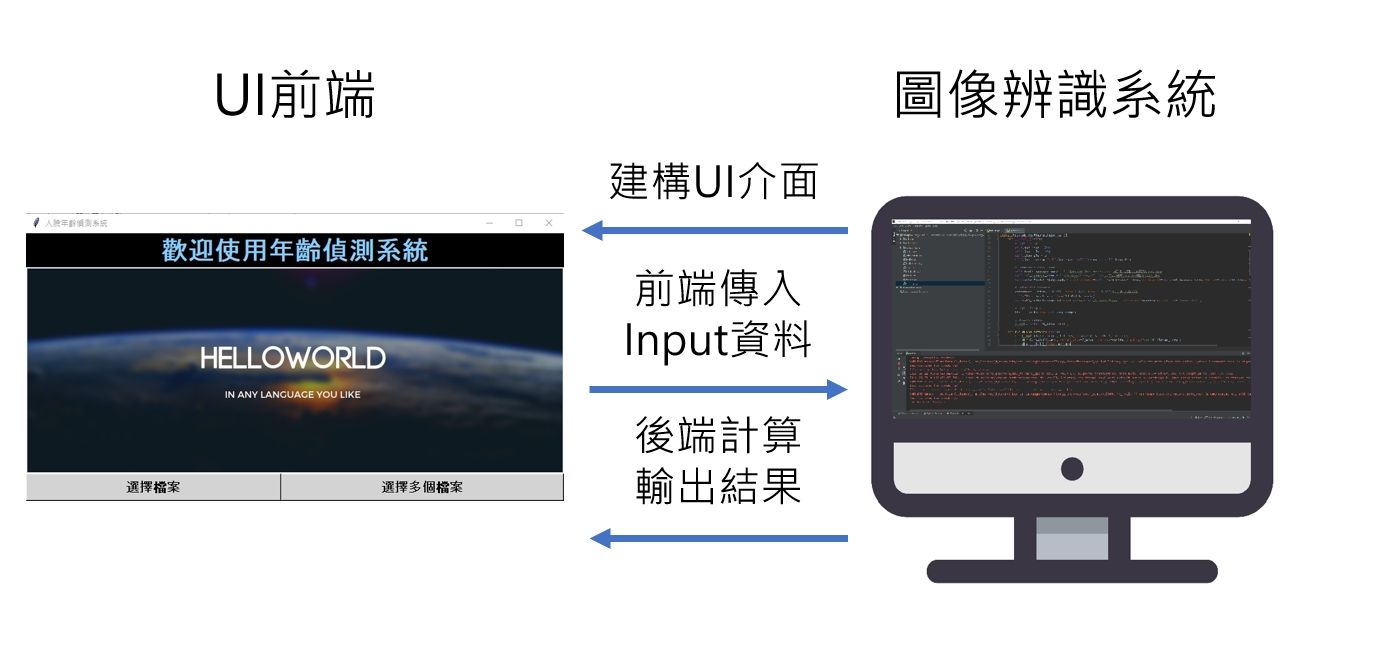
\includegraphics[scale=0.4]{image/UIandSystem.jpg}%
        \end{center}
        \caption{UI and System.}
        \label{fig:1}
    \end{figure}
\vspace{5.0cm}
\section{Product Functions}
UI前端會送出使用者所選擇圖片之路徑,傳至後端人臉辨識系統,經過人臉辨識模組後傳回圖片以及該圖片人物的年齡。流程圖如下:\\
    \begin{figure}[htb]
        \begin{center}
            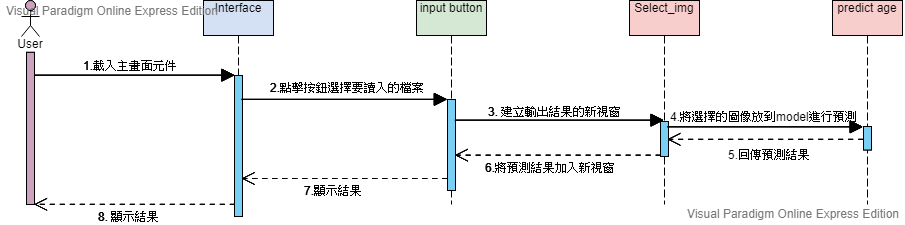
\includegraphics[scale=0.5]{image/sequenceDiagram.png}%
        \end{center}
        \caption{sequence Diagram(使用UML線上工具繪製)}
        \label{fig:2}
    \end{figure}

\section{User Classes and Characteristics}
本系統只為人臉辨識中的其中一環,提供給其他整合人臉辨識系統的專案其中一項功能,
同時,也提供操作的介面讓專案測試人員能選擇圖片去測試系統人臉辨識完成度。\\

\section{Operating Environment}
\begin{itemize}
    \item Windows 10 作業系統
    \item Python 3.6
    \item TensorFlow Background
\end{itemize}

\section{Design and Implementation Constraints}
由於Project製作時程不夠長,加上目前所學的技術限制,會有以下問題不支援
\begin{itemize}
    \item DataSet資料不夠齊全,每個資料類型也不太平均
    \item 準確率沒辦法到達100\%
    \item 沒有辦法精準的算出歲數,只能歲出歲數區間
    \item 預測速度不夠快,要一次跑多張圖時特別明顯
\end{itemize}

\section{Assumptions and Dependencies}
\begin{tabular}{ |l|l| }
    \hline
    \multicolumn{2}{|c|}{額外的安裝包} \\
    \hline
    datetime & Paul Robinson \\
    \hline
    numpy & Lucas Radebe \\
    \hline
    sklearn.metrics.accuracy_score & 測量分類準確度 \\
    \hline
    keras & 卷積網路運算 \\
    \hline
    csv & 讀取CSV檔案 \\
    \hline
    cv2 & opencv圖像處理 \\
    \hline
    PIL.Image & pillow圖像處理 \\
    \hline
    tkinter & python UI函式庫 \\
    \hline
\end{tabular}

\chapter{External Interface Requirements}

\section{User Interfaces}
\vspace{0.9cm}
\begin{enumerate}
    \item 主介面如 Fig.\,\ref{fig:1} 所示,包含封面頁,以及可以選擇測試檔案的按鈕,有分為選擇檔案和選擇多個檔案。\\
    \begin{figure}[htb]
        \begin{center}
            \includegraphics[scale=0.7]{image/UiHomePage.png}%
        \end{center}
        \caption{UI Home Page.}
        \label{fig:1}
    \end{figure}
    \vspace{7.0cm}
    \item 按下選擇檔案按鈕則開啟一個資料夾視窗,可選擇一個jpg檔案和png檔案,如 Fig.\,\ref{fig:2} 所示\\
    \begin{figure}[htb]
        \begin{center}
            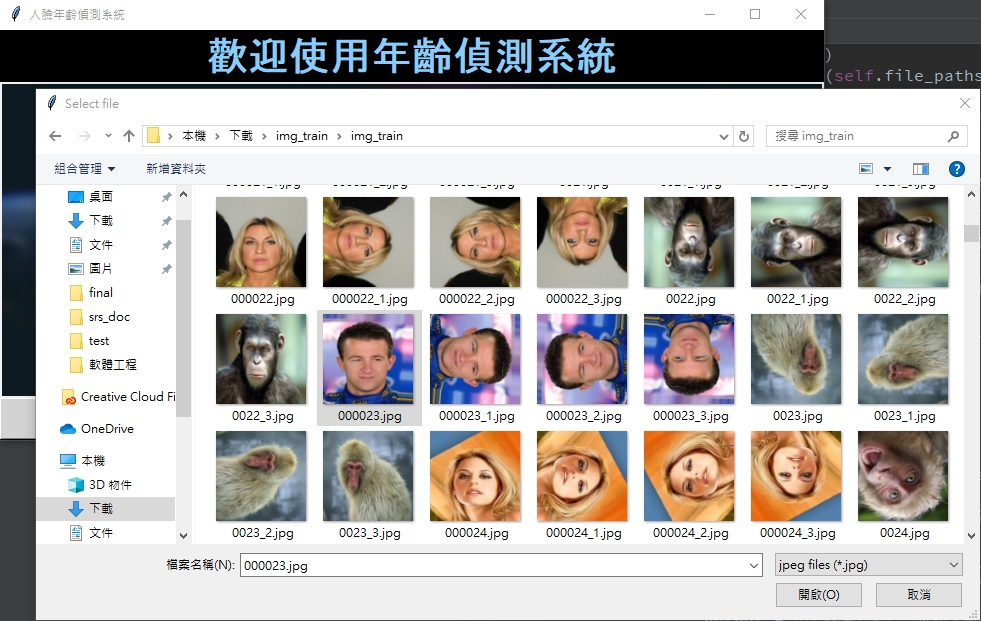
\includegraphics[scale=0.6]{image/UiSelectFileOne.png}%
        \end{center}
        \caption{UI Select One File Window.}
        \label{fig:2}
    \end{figure}
    \vspace{7.0cm}
    \item 按下選擇多個檔案按鈕同樣可開啟一個資料夾視窗,可選擇多個jpg檔案和png檔案,如 Fig.\,\ref{fig:3} 所示\\
    \begin{figure}[htb]
        \begin{center}
            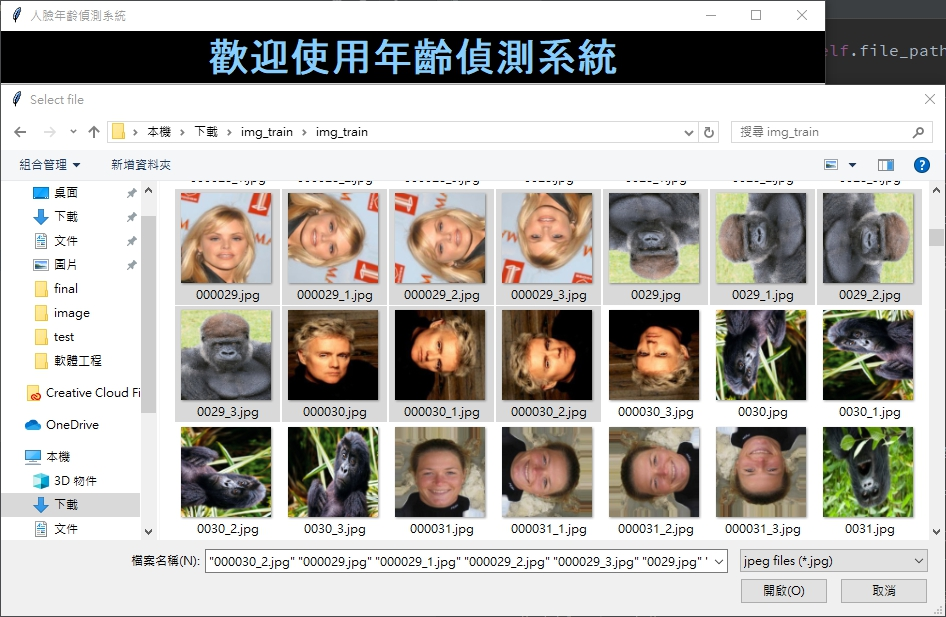
\includegraphics[scale=0.6]{image/UiSelectFileMulti.png}%
        \end{center}
        \caption{UI Select Multi File Window.}
        \label{fig:3}
    \end{figure}
    \vspace{7.0cm}
    \item 選擇了圖片後按下開啟,等待系統回應幾秒鐘會回傳該圖片以及判斷的年齡區間,以及左下角有離開程式的按鈕,按下就結束執行。中間有一個看新圖片的按鈕,按下可回到主畫面,新再跑一次。右下角則是只有一開始點擊開啟多個檔案才可以案的按鈕,意思是繼續查看剛剛你所選的下一張圖片,如 Fig.\,\ref{fig:3} 所示\\
    \begin{figure}[htb]
        \begin{center}
            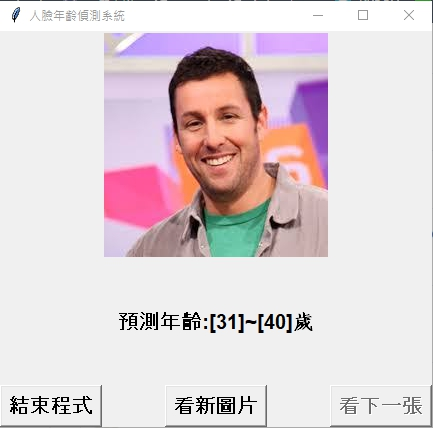
\includegraphics[scale=0.8]{image/UiResponse.png}%
        \end{center}
        \caption{UI Response.}
        \label{fig:3}
    \end{figure}
\end{enumerate}

\section{Hardware Interfaces}
\begin{enumerate}
    \item CPU: intel i5-6200U5
    \item Memory: 8GB
\end{enumerate}

\section{Software Interfaces}
\begin{enumerate}
    \item Windows 10 64 bit
    \item Python 3.6
    \item TensorFlow Background
    \item Keras API
\end{enumerate} 

\chapter{System Features}
\section{Description and Priority}
我們的系統是一個利用人類臉部來偵測年齡的系統,以優先度來說,偵測年齡的準確度絕對是最重要的,因為這也是這個系統最主要的功能,但受限於dataset資料量不夠大及一些技術上的限制,沒辦法達成更高的準確度。其次是執行速度與UI界面,因為對於一般使用者來說,快速的執行速度與美觀的界面也是會讓人想繼續使用你的程式的原因之一

\section{Stimulus/Response Sequences}
Case1:
    \begin{enumerate}
    	\item 進入系統UI主畫面
    	\item 點擊選擇檔案按鈕,選擇一張圖片
    	\item 載入model進行預測
    	\item 將預測結果顯示在UI界面上
	\item 按結束程式結束或著按看新圖片按鈕回到第一步繼續執行
    \end{enumerate}
Case2:
    \begin{enumerate}
    	\item 進入系統UI主畫面
    	\item 點擊選擇多個檔案按鈕,選擇多張圖片
    	\item 載入model進行預測
    	\item 將預測結果顯示在UI界面上,點及下一張可繼續預測所選的下一張圖片
	\item 按結束程式結束或著按看新圖片按鈕回到第一步繼續執行
    \end{enumerate}

\section{Functional Requirements}
載入圖片
    \begin{itemize}
	    \item 點擊選擇檔案可彈出檔案視窗
	    \item 可選擇任意一個jpg或png檔讀進來
	    \item 點擊選擇多個檔案,同樣可彈出檔案視窗
	    \item 可一次選擇多個jpg或png檔案讀進來
    \end{itemize}
分析圖片
    \begin{itemize}
	    \item 運用分析好的model自動對圖片做預測
    \end{itemize}
輸出結果
    \begin{itemize}
	    \item 顯示預測分析出的年齡範圍及resize後的圖片
	    \item 按結束程式可終止程式
	    \item 按看新圖片可回到主畫面重新進行選擇
	    \item 若為多張照片,可按下一張來繼續看所選圖片的預測結果
    \end{itemize}


\chapter{Other Nonfunctional Requirements}

\section{Performance Requirements}
年齡偵測準確率:
    \begin{itemize}
	    \item 基於現有技術和dataset的限制,我們會將準確率控制在60\%以上
    \end{itemize}
穩定性:
    \begin{itemize}
	    \item 運用穩定的編譯環境及防呆機制完善的UI系統介面,將出錯機率降到最低
    \end{itemize}
執行效率:
    \begin{itemize}
	    \item 透過對testing程式碼的不斷優化,雖然預測時間還是偏長,但相較於以前已有逐漸改善
    \end{itemize}
可讀性:
    \begin{itemize}
	    \item 將程式碼模組化,並寫上註解,方便之後需要時能快速理解並能夠做局部修改
    \end{itemize}


\section{Safety Requirements}
    \begin{itemize}
	    \item 只讀單張圖片、或是讀到了多張圖的最後一張,會直接把下一張的button鎖起來,避免程式繼續執行而報錯
	    \item 選擇檔案時,只會選到jpg檔或png檔
	    \item 打開檔案視窗時,如果按下取消,會直接回到主畫面,不會跳出取不到路徑值的錯誤訊息
	    \item 對讀進來的圖片重新resize,讓圖片的shape不會不相容
    \end{itemize}

\end{CJK}
\end{document}
